\chapter{\label{cpt:architecture}Architecture}

The architecture of \Amber\ is defined in terms of modules and the messages
they use to communicate. A global architecture is depicted in
Figure~\ref{fig:global-architecture}.

In the Section~\ref{sct:modules} the modules are described in detail and in
Section~\ref{sct:messages} the messages connecting them are defined. The data
types used in the system are described in Section~\ref{sct:types}.

\begin{figure}
    \centering
    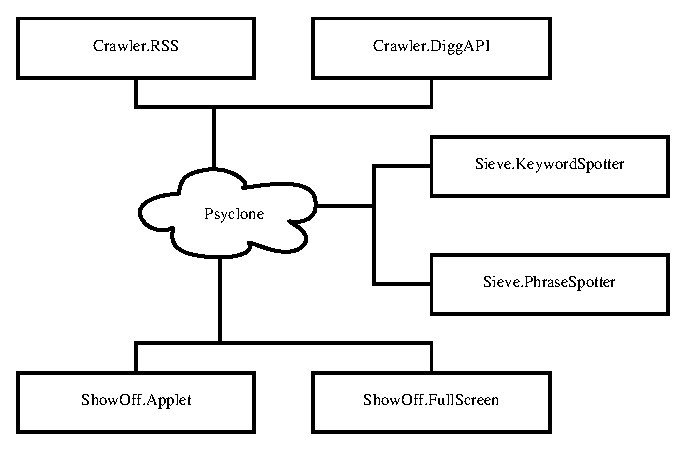
\includegraphics{image/global-architecture}
    \caption{\label{fig:global-architecture}Global \Amber\ architecture, the names are Psyclone module names}
\end{figure}

\section{\label{sct:modules}Modules}

A complete \Amber\ system will comprise at least three modules running at the
same time; there is a Crawler module, a selector module called Sieve and a
display called ShowOff. The modules are separate executables with their own
life-cycles and resources. Since TCP/IP is used, the executables don't need to
be on the same machine to communicate.

Every module has a specified interface through which communication with
Psyclone is handled.

\subsection{Crawler modules}

When the Crawler is started, it will create one of the available handlers
(depending on what is specified on the command line or what is set as default
during build time). 

It also creates an AirBrush instance to communicate with Psyclone via
Java\-Open\-AIR. The module name announced to Psyclone is `Crawler.' plus the
name of the handler, so `Crawler.RSS' in case of the RSS handler.

After connecting with Psyclone, the handler can get its parameters stored in
the psySpec file and go to work. It will post stories with type `Story'  on the
whiteboard `WB.Stories'.

\subsubsection{RSS}

The RSS crawler module will be fairly straightforward. There are actually quite
a few good RSS parsers around for Java, the only thing the crawler should do is
getting the stories from the RSS feeds along with meta-information and store it
on the whiteboard.

Although the module is called RSS, it can also handle Atom feeds, which is also
quite a popular format.

\begin{module}{Crawler.RSS}
  \trigger{Feed.*}{WB.Control}
  \post{Story}{WB.Stories}
\end{module}

\subsubsection{DiggAPI}

Digg is a website which lets users submit stories found on the web. Other users
then moderate the submissions either by `digging' or `burying' a story. A story
with a lot of `diggs' is a popular one. The nice thing about Digg is that it
actually does a lot of preprocessing work for the \Amber\ system.

Digg
announced\footnote{\url{http://diggtheblog.blogspot.com/2006/07/digg-labs-launches-alpha.html}}
that they will publish a public API within the next months. If time allows, a
DiggAPI module is created.

\begin{module}{Crawler.DiggAPI}
    \post{Story}{WB.Stories}
\end{module}

% \subsubsection{BloggerDataAPI}
% 
% One of the larger weblog hosters is Google with their Blogger service. There
% is an API available to get information from it.
% 
% \begin{module}{Crawler.BloggerDataAPI}
%   \post{Story}{WB.Stories}
% \end{module}


\subsection{Sieve modules}

All analysis modules, or sieves, will get a trigger from a new story on the
whiteboard WB.Stories. They analyse it and if there is anything to say about
the story, a Analysis message is sent to the whiteboard WB.Analyses containing
its judgement on the story.

The contents of this message is specified in Section~\ref{sct:messages}.

Analysis modules may take any time they like to come to a verdict, but it is
possible that a story has already disappeared from the visualization if the
response is very late.

Since all modules employ the same external behaviour, the Psyclone
specification is the same for every one of them.

\begin{module}{Sieve.???}
    \trigger{Story}{WB.Stories}
    \post{Analysis}{WB.Analyses}
\end{module}

\subsection{ShowOff modules}

The ShowOff modules are visualizers which combine the crawled stories from the
Crawler with the analyses from the Sieve modules.

\begin{module}{ShowOff.???}
    \trigger{Story}{WB.Stories}
    \trigger{Analysis}{WB.Analyses}
\end{module}

\subsubsection{Full screen}

The full screen application will display a lot of information and is there to
be looked - not glanced - at. It should be possible to let it do its job
autonomously, just showing a pretty picture, or to be interactive.

\subsubsection{Ambient applet}

The ambient applet will display a very easy to understand image (a glance at it
should be enough) of the status of the page it is on. I.e. if the page is a
weblog, it should display subject information on that weblog, if it is on the
page of a thread of a forum, it displays the flow of the discussion.



\section{\label{sct:messages}Messages}

There are a few message types in the system. Two of which must be defined
system-wide because they are used in the communication between modules.

\subsection{\label{sct:messages:story}Message type `Story'}

The Story message is only posted to the whiteboard `WB.Stories' and only by
Crawler modules.

The message content is a \ac{YAML}\footnote{\url{http://www.yaml.org/}} document
which represents the storyData field inside the Java counterpart of the
message. It contains at least the properties `URI' (to identify the story,
GUIDs are RSS specific and cannot be used), `Author', `Title', `Story-Content'.

It may also contain `Publication-Date' (which is the date of publication in
Internet~Message~Format\cite[Section~3.3]{RFC2822}), `Kind' and other fields.

An example of a YAML document containing Story data:

\begin{verbatim}
---
URI: http://ijsland.luijten.org/2006/09/12/skyr-wasdanou/
Author: Christian Luijten
Title: Skyr... Wasdanou?
Publication-Date: Tue, 12 Sep 2006 21:03:54 +0000
Kind: weblog-posting
Story-Content: >
  Een van die dingen die bij een onbekende cultuur horen zijn de
  eetgewoonten. Elk land heeft zo z’n producten die je nergens
  anders kan krijgen. IJslands nationale zuivelproduct heet Skyr,
  elke oma kan het maken, al is het nogal een hoop werk. Daarom is
  het lange tijd (lees: gedurende de jachtige periode na de tweede
  wereldoorlog toen de Amerikanen hier de boel kwamen ophaasten)
  in ongebruik geraakt, maar op een gegeven moment kwam de vraag
  toch weer terug en zijn een aantal zuivelproducenten het
  industrieel gaan produceren.
\end{verbatim}

\subsection{Message type `Analysis'}

Analysis typed messages are posted on the `WB.Analysis' whiteboard only by
Sieve modules. They contain information about stories present on the
`WB.Stories' whiteboard.

The content of these messages is also YAML format. Stories and Analysis
messages are coupled through their `URI' fields, so this must be present.

An example of a message issued by an analysis module checking for the topic
`Zuivel' (which means dairy products in Dutch):

\begin{verbatim}
---
URI: http://ijsland.luijten.org/2006/09/12/skyr-wasdanou/
Topic: Zuivel
Relation-Strength: 1.0
Author-Strength: 0.1
\end{verbatim}

Its `Relation-Strength' suggests high relevance of the content with the topic.
However, the `Author-Strength' suggests that the author isn't an authority in
the field.

Every analysis module sends a message to the whiteboard if it thinks it is
relevant. It is thus possible that the same URI will get multiple analysis
results or nothing at all, the visualizer module must cope with this and merge
the available information.



\input{04.3-types.inc}

